\subsection{Circuit}

	\subsubsection{Intégration Matérielle}

		\paragraph{Circuit en lui-même}
			Notre circuit sera donc bien composé de deux parties, chacune constituée d'un panneau de médium monté sur un cadre en tasseaux.
			D'autres problématiques ont fait leur apparition en cours d'étude du projet et c'est ainsi que l'on intègrera des perçages pour la fixation des feux et le passage des fils, mais surtout pour l'intégration des fameux "caches" permettant d'isoler visuellement les "rues".\\

			Les panneaux seront peints en noir et recouverts de scotch d'électricien blanc représentant les lignes. Nous obtenons ainsi un rapport de contraste idéal (noir mat du bois et blanc brillant du ruban adhésif). Le plan à l'échelle de la piste est le suivant :
			\illu{CIRCUIT.pdf}{Plan à l'échelle de la piste}{0.065}

			\vspace{15pt}

			Y apparaissent les lignes, code-barres et caches (en gris plein) évoqués dans le dossier. Les rayons de courbure sont de 75mm, et l'espacement entre les voies et divers obstacles de 220mm.\\

			Un plan contenant toutes les côtes sera produit et pourra être "recopié" à l'aide de simple matériel scolaire (compas, règle, équerre) sur les panneaux avant d'être recouvert par le ruban adhésif.\\

			Les capteurs ILS seront fixés aux panneaux.\\
			On prévoiera des vis "dépassant" aux emplacements appropriés afin de pouvoir y "emboiter" les feux.\\

			Le câblage des capteurs et des feux sera solidaire de chaque partie, et passera par des trous prévus à cet effet dans les tasseaux pour converger en un "faisceau" terminé par un connecteur pour chacune des deux parties. Un connecteur sera présent du côté de chaque feu avec suffisemment de longueur de câble pour pouvoir facilement procéder à l'installation desdits feux.

			Voici à quoi ressemblerait le circuit (les petits éléments ne sont pas visibles):
			\illu{CIRCUIT2.png}{Modélisation 3D du circuit}{0.4}

		\paragraph{Carte électronique}

			La carte aura pour but de servir d’interface entre la carte FPGA et les composants électroniques du circuit (LEDs des feux bicolores et capteurs ILS).\\
			Comme évoqué précédemment, deux faisceaux de câbles terminés par des connecteurs arriveront sur cette carte (un pour chaque moitié de circuit). Ces faisceaux seront constitués de dix fils correspondant à :

			\begin{itemize}
				\item Masse feu 1
				\item Masse feu 2
				\item LED verte feu 1
				\item LED rouge feu 1
				\item LED verte feu 2
				\item LED rouge feu 2
				\item Retour ILS 1
				\item Retour ILS 2
				\item Alimentation ILS 1
				\item Alimentation ILS 2
			\end{itemize}

			Les cartes FPGA Basys 2 utilisées à l’IPSA disposent de quatre ports d’extensions dits « pmod » \cite{bib22}. Ces ports ont un format on ne peut plus standard : connecteurs femelles espacés d’un dizième de pouce (2,54mm).\\
			Chaque connecteur fournit 6 contacts :\\
			\begin{itemize}
				\item Une sortie 3,3V
				\item Une Masse
				\item 4 ports d’entrée/sorties directement mappés sur le FPGA.
			\end{itemize}

			\illu{pmod.png}{Illustration d'un port "pmod" \textbf{\textit{(source : Digilent)}}}{0.4}

			Les LEDs seront commandées par des ports du FPGA configurés en sortie.\\
			Pour ne pas tirer trop de courant sur ces ports (qui ne sont pas fait pour : il sont conçus pour produire des signaux et non des alimentations) et pouvoir fonctionner aussi bien en logique TTL que CMOS, nous passerons par un circuit intégré de la famille 74HC (\textbf{attention à bien différencier la série 74HC de la série 74HCT que nous serons également amenés à utiliser : elles n'ont pas les mêmes tensions de référence !}). 
			Ces portes logiques reposent sur la technologie « collecteur ouvert » et peuvent donc être utilisés comme des transistors de faible puissance. Les entrées logiques correspondent aux bases, les sorties aux émetteurs et l’alimentation du composant (Vcc) aux collecteurs.\\

			La datasheet \cite{bib24} nous apprend qu’ils peuvent fournir jusqu’à 50mA en sortie sur l’ensemble des sorties. En répartissant 4 LEDs par circuit logique et en utilisant ces dernières à 10mA (largement suffisant pour des LEDs  haute luminosité), nous restons en dessous de cette limite même lorsque les 4 LEDs sont allumées simultanément (ce qui en théorie ne devrait pas être le cas).
			Nous utiliserons le 74HC04 qui est un sextuple inverseur (seul 4 éléments seront utilisés). Ainsi, en plaçant un « 1 » (3.3V ou 5V : les deux fonctionnent puisque le composant reconnaît une valeur haute à partir de 2,3V) en entrée, nous obtenons 0V en sortie. En y plaçant un « 0 » (0V), nous obtenons un 3.3V jusqu 20mA par sortie pour un total de 50mA maximum ! Le tout sans jamais prélever plus d’un milliampère en entrée (et donc en sortie du FPGA).\\

			Les sorties du 74HC04 pourront être directement connecés aux anodes des LEDs via une résistance appropriée (150$\Omega$ pour une LED rouge à 1,8V de chute et 100$\Omega$ pour une LED verte à 2,3V de chute).\\


			L’acquisition des états des capteurs ILS est encore plus simple : les ILS étant de simples interrupteurs, on placera l’une de leurs bornes à la masse et on connectera l’autre à une entrée du FPGA en intercalant une résistance de pull-up placée à 3.3V.\\
			Ainsi, la carte FPGA verra un signal stable au niveau haut qui ne passera au niveau bas que lorsqu’un aimant excite le capteur.\\

			Nous pourrions simplifier et « sécuriser » le circuit en intégrant une partie de la logique de fonctionnement de manière électronique (penser le circuit pour que deux LEDs du même feu ne puissent-être allumées simultanément, par exemple), mais ceci irait à l’encontre de la vocation pédagogique du système et limiterait sa capacité d’évolution.\\

			Nous utiliserons de simple connecteurs sécables standard pour connecter le circuit à la carte Basys 2. Ainsi, on pourra directement « enficher » les deux cartes. Mais si l’IPSA venait à acheter de nouvelles cartes FPGA, l’utilisation de simples câbles « strips » permettra de se dispenser de refaire la carte.\\

			\illu{secable.png}{Illustration d'un connecteur sécable 0.1'' standard \textbf{\textit{(source : Gotronic)}}}{0.5}

			Nous aurions voulu mettre en place un système permettant de s’assurer que la carte ne peut être branchée que « dans le bon sens » (avec des connecteurs asymétriques par exemple) mais nous dépendons des connecteurs de la Basys 2 et ne pouvons implémenter cette sécurité. Il faudra donc être extrêmement attentifs à l’utilisation qui sera faite des cartes pour ne craindre aucun dommage (un analyse rapide des schémas nous montre cependant que peu de mal peut être infligé par un mauvais branchement). Surtout, la carte Basys2 est équipée sur ses ports pmod de diodes et résistances de protection \cite{bib23}.

	\subsubsection{Intégration Logicielle}

		Le cas du feu de circulation s'adaptant au trafic est l'exemple type de la logique dite de "l'automate fini". La littérature ne manque pas à ce sujet et nous avons même eu l'occasion de l'étudier au cours de notre cursus.\\

		La logique VHDL \nomenclature{VHDL}{VHSIC1 Hardware Description Language : langage destiné à la programmation de cartes FPGA.} est particulièrement adaptée à ce type de problématique et offre la possibilité de coder un certain nombre d'états et de définir les conditions et modalités de changement d'état.\\

		Dans notre cas, nous compterions trois états:
		\begin{itemize}
			\item \textbf{Etat 0} : Tous les feux au rouge.
			\item \textbf{Etat 1} : Couple de feux A au rouge et couple B au vert.
			\item \textbf{Etat 2} : Couple de feux B au rouge et couple A au vert.
		\end{itemize}

		\vspace {12pt}
		Une succession classique d'états serait 0->1->0->2->0->...\\
		Pour simplifier l'organisation du programme, nous pourrions créer un état intermédiaire entre 1 et 2, identique à l'état 0.\\

		Un diviseur d'horloge permettrait de générer des événements à intervalles réguliers afin de cadencer le changements d'états.\\
		Les capteurs eux-mêmes pourraient générer un événements (sur un front montant de l'entrée logique à laquelle ils sont branchés par exemple) qui, si un certain nombre de conditions sont réunies, anticiperaient le changement d'état (si une voiture se présente à un feu rouge et qu'aucune ne "profite" des feux verts, alors il est plus logique d'inverser cet état).

\subsection{Robot}

	\subsubsection{Intégration Matérielle}

		\paragraph{Ensembles propulsifs}

			Les deux "ensembles de propulsion" seront placés à l'arrière du robot. Une simple bille multidirectionnelle sera placée l'avant pour assurer la stabilité du robot.\\

			Le choix de notre motoréducteur fut basé sur un ensemble de critères :
			\begin{itemize}
				\item Le motoréducteur doit nous permettre d’atteindre une vitesse de pointe minimum de 15 cm/s (environ 70 tours par minute pour une roue de diamètre 4cm).
				\item Le motoréducteur devrait bénéficier d'un couple "confortable" pour les manoeuvres du robot.
				\item Le moteur ne devra pas être surdimensionné de manière à maîtriser la consommation d’énergie.
				\item On se munira du moteur le moins cher répondant aux critères précédents.
				\item Nous désirions aussi dans la mesure du possible trouver un moteur possédant un encodeur intégré, cependant ce critère ne correspond pas à un critère d’arrêt.
			\end{itemize}

			Nous avons estimé le couple minimum nécessaire à 0,01Nm par moteur (en effectuant le calcul pour différentes masses et inclinaisons de la piste).\\

			Il a ensuite fallu composer avec l'offre limitée présente sur le marché "semi-amateurs".\\

			Nous avons finalement sélectionné le motoréducteur "High-Power" de Pololu dans sa version proposant un taux de réduction de 298 pour 1.
			Ce moteur propose les caractéristiques suivantes :\cite{bib8} \\

			\begin{itemize}
				\item Couple de blocage de 0,5Nm
				\item Vitesse à vide sous 6V de 100 tours par minute
				\item Courant à couple maximum de 1.6A (soit 400mA maximum en utilisation normale)
			\end{itemize}


			Ce motoréducteur est associable avec une roue et un encodeur du même constructeur qui forment un ensemble fonctionnel et simple à implémenter. Nous y associerons un support PVC adapté pour la fixation.\\
			Notons qu'un seul des deux moteurs sera équipé d'un encodeur, deux étant superflus et évidemment plus chers.

			Le motoréducteur est équipé de deux fils d'alimentation. Nous les connecterons à la carte-mère au travers d'un bornier. Un double pont en H intégré L293D (comprenant les diodes de roue libre \cite{bib17}) permettra de faire le lien entre le signal PWM généré par le BBG (3.3V limité à une vingtaine de milliampères) et le moteur (que l'on alimentera directement sur la batterie, le signal PWM étant donc adapté sur une base 7.2V). Trois sorties seront donc utilisées sur le BBG pour chacun des deux moteurs : une PWM pour gérer la puissance transmise au moteur, et deux digitales pour le sens de rotation. Ces signaux (de 3.3V) pourront-être directement transmis au double pont en H (le L293D ayant une tension "niveau haut" de 2,3V \cite{bib17}). Nous compterons deux sources d'alimentation pour le pont en H : une alimentation de 5V pour le circuit logique et une alimentation directe sur la batterie (on pensera à intégrer deux condensateurs pour filtrer le bruit dû aux moteurs). Les signaux logiques viendront directement du BBG.\\

			Pour plus de détail, voir \ref{carteMere} (page \pageref{carteMere}).\\

			L'encodeur peut, d'après sa fiche technique \cite{bib9} fonctionner en 3.3V. Cependant, la diode émettrice IR perdra alors de son intensité. Nous procéderons donc à une expérience pour définir si ce fonctionnement en "sous régime" de la diode est satisfaisant. Dans le cas contraire, nous alimenterons l'encodeur en 5V et procéderons à une division de tension sur le signal de sortie avant de le transmettre au BBG, pour ne pas endommager ce dernier. Notons qu'un seul des deux "canaux" de l'encodeur nécessitera d'être connecté au BBG étant donné notre besoin de précision. Ainsi, la carte- mère devra comprendre un connecteur trois contacts dédié à l'encodeur : deux contacts serviront simplement à l'alimentation, et le troisième (le signal) sera connecté à l'une des entrées du BBG permettant l'utilisation du module eQEP (voir \ref{eQEP}).

		\paragraph{Carte Réflecteurs Optiques}\label{integrationReflecteurs}

			Rappelons que nous utiliserons les entrées analogiques du BBG pour effectuer l'acquisition des données du capteur, et que ces dernières sont limitées à 1.8V (voir \ref{solutionSuiviLigne}, page \pageref{solutionSuiviLigne}).

			La datasheet du TCRT5000 \cite{bib7} nous apprend que la LED émettrice possède une tension directe de 1.25V et n'accepte que jusqu'à 60mA.
			Afin de ne pas surcharger la sortie à 1.8V fournie par le BBG (qui ne fournit pas plus de 50mA), nous alimenterons les LEDs en 5V via une résistance de 120$\Omega$, faisant ainsi traverser la LED par $\frac{5-1.25}{120}=31mA$, ce qui est idéal (intensité IR\nomenclature{IR}{Infra-Rouge} suffisamment élevée sans risquer "d'éblouir" les autres capteurs ou de griller la LED).\\

			On connectera le collecteur du phototransistor à la ligne 1.8V au travers d'une résistance de pull-up de 2.7k$\Omega$, la valeur la plus élevée de résistance nous permettant d'assurer un courant de collecteur de 5mA (comme recommandé dans la datasheet). Nous choisissons la valeur la plus élevée afin de limiter la consommation en courant, mais surtout d'augmenter la sensibilité du capteur (il sera ainsi plus facile au phototransistor de "tirer" la tension vers le bas).\\

			Nous avons donc le schéma de principe suivant :
			\illu{reflecteur.pdf}{Schéma de principe d'un réflecteur optique}{2}

			Ce schéma sera reproduit sept fois sur une carte dédiée, qui sera placée à l'avant du robot, parfaitement centrée et placée quelques millimètres au dessus de la piste (la datasheet nous apprend que la distance de fonctionnement idéale entre le capteur et le support est de 2.5 mm, avec un domaine de fonctionnement allant de 0.2 à 12mm).\\
			
			Sachant que la ligne au sol aura une épaisseur de 15mm, nous placerons les trois capteurs centraux de manière à ce que, lorsque le capteur central est placé au milieu de la ligne, il ne manque que 2 à 3mm aux deux autres pour y arriver . Les autres capteurs pourront avoir un écartement légèrement plus élevé :

			\illu{espacementReflecteurs.pdf}{Espacement des réflecteurs optiques}{0.8}

			Notons que la distance exacte entre les capteurs ne pourra être précisément définie que par l'expérience. En effet, nous n'avons aucune indication quant à la largeur du champ de détection du capteur.\\

			Nous connecterons la carte au moyen d'une nappe HE10 à 10 connecteurs.\\

			Le schéma électronique et les gerbers du circuit imprimés sont disponibles en annexe \ref{schemasCarteReflecteurs} (page \pageref{schemasCarteReflecteurs})

		\paragraph{Carte-Mère}\label{carteMere}

			La carte mère est le circuit imprimé permettant de relier véritablement les actions "logicielles" aux actions réelles. Les contraintes pour cette carte sont simples :
			\begin{itemize}
				\item De taille raisonnable, soit de la taille bu BBG
				\item Ne pas intégrer directement les composants ayant un impact sur l'environnement du robot (moteur, LEDs...), pour qu'en cas de défaillance, ainsi que toujours dans un esprit de modularité et d'amélioration continue, un élément soit interchangeable rapidement, par le biais de connecteurs standards.
				\item Facilement intégrable au BBG. L'idée est vraiment de réaliser un shield enfichable simplement.
			\end{itemize}
			

			Ce shield intègre une prise standard de type Barrel jack, et peut être alimenté par toute source de tension supérieure à 7V. 
			\illu{barrelJack.jpg}{Embase Barrel Jack \textbf{\textit{(source : Conrad.fr)}}}{0.1}
			En effet, les moteurs demandant plus de 5v, il fallait trouver un moyen d'abaisser cette tension. Nous avons donc opté pour un régulateur de tension à découpage, réglé à 5v. Le principe est simple : Un PWM est généré avec comme tension haute la tension d'entrée. En modulant cette impulsion et en faisant passer le signal par un filtre passe-bas, on lisse le signal à une valeur donnée (ici, 5v). L'inconvénient de ce genre de régulateur par rapport aux régulateurs est qu'ils nécessitent plusieurs composants. Mais le principale avantage réside dans leur rendement : jusqu'à 95\% \cite{bib25} ! Un régulateur de tension classique "tranforme la tension d'entrée en excès" en chaleur. Ainsi, pour une entrée à $7,2v$ et une sortie à $5v 1A$, la puissance dissipée est de $P = (V_{in} - V_{out}) \times I = (7,2 - 5) \times 1 = 2,2 W$ ! De plus, sachant que l'intensité en entrée est la même que l'intensité en sortie, on obtient un rendement $R = \frac{V_{out}}{V_{in}} = \frac{5}{7,2} = 69\%$. Une alimentation à découpage, bien qu'un peu plus onéreuse, permettra donc d'augmenter considérablement l'autonomie.\\
			La carte BBG n'étant pas capable de fournir une intensité maximum élevée, nous avons décidé d'utilisé un sextuple inverseur (6 portes Nand) à haute impédence d'entrée afin d'agir comme un buffer : le 74HCT04. Ce composant est capable de fournir l'intensité nécessaire à nos 5 LEDs,ces dernières étant en série avec des résistances adaptées.\\  
			Nous avons également inséré, avant et après l'alimentation, en parallèle, des condensateurs. Ceux-ci permettent de s'assurer que la tension est bien stable en supprimant les hautes fréquences. Etant donné que des intensités relativement élevées (dûes aux moteurs) seront mises en jeu, il est probable que des pics de tension apparaissent. Même si ce pic n'est pas démesuré, il pourrait tout de même endommagé la carte.\\

			Nous avons également décidé d'intégré un interrupteur à levier de type On/Off, afin d'économiser la batterie lorsque les moteurs ne sont pas nécessaires, et ainsi gagner en autonomie. Nous avons également inclu un bouton poussoir à impulsion (de type NO \nomenclature{NO}{Normally Open, Normalement ouvert}(On)/Off, selon les notations normalisées). Ce dernier démarrera la séquence de test, permettant ainsi de positionner le robot sur le circuit avant de commencer les tests.\\
			Les deux boutons sont accompagnés en dérivation de condensateurs. En effet, lors d'un changement d'état d'un interrupteur, le signal ne passe pas d'un état à un autre (de HAUT/HIGH à BAS/LOW ou inversement) immédiatement et parfaitement. Il y a une phase de transition qui, si elle n'est pas géré physiquement ou logiciellement, peut causer de graves problèmes, tel qu'un appui multiple, pouvant lancer plusieurs fois la séquence, entrainant des perturbations et pouvant potentiellement endommager le robot et/ou la carte. On parle de "debouncing", comme le présente la figure suivante :
			\begin{figure}[H]
				\centering
				\begin{subfigure}[h]{0.45\textwidth}
			        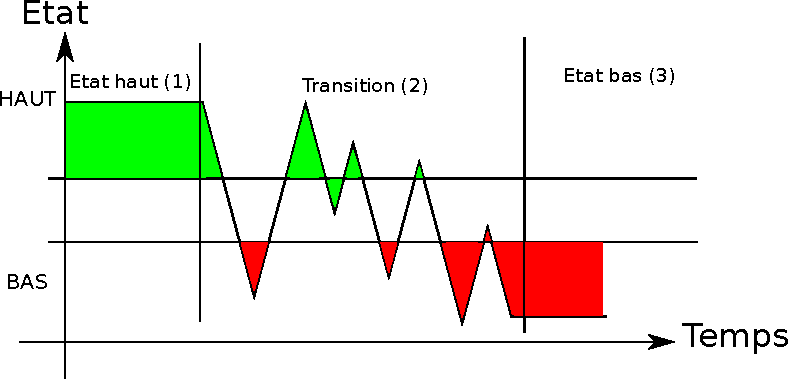
\includegraphics[width=\textwidth]{Graphics/btnNoDebounce.pdf}
			        \caption{Sans condensateur}D
			    \end{subfigure}
			    ~
			    \begin{subfigure}[h]{0.45\textwidth}
			        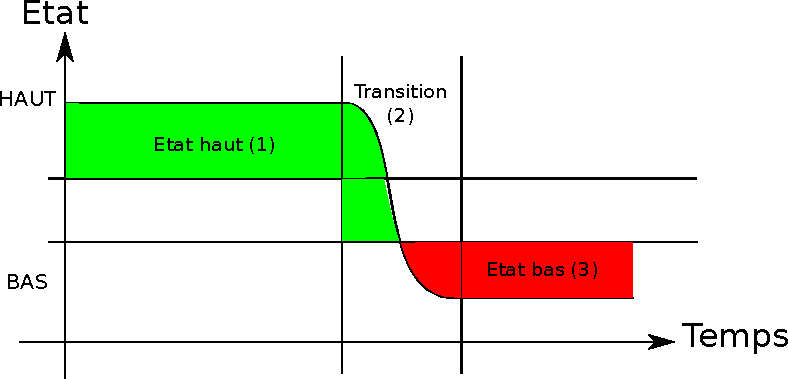
\includegraphics[width=\textwidth]{Graphics/btnDebounce.pdf}
			        \caption{Avec condensateur}
			    \end{subfigure}
			    \caption{Schéma de l'état d'un signal après l'ouverture d'un interrupteur}
			\end{figure}
			Grâce à ces schémas, on se rend rapidement compte de l'importance d'un simple composant passif. Dans le cas (a), le controlleur pourrait croire à de multiples pressions de l'interrupteur, pouvant engendrer des dommages au système mécanique, aussi bien qu'au système électrique. Dans le cas (b), le signal est continu et lissé. Il s'agit finalement d'un simple filtre passe-bas, puisqu'on a effacé toutes les hautes fréquences parasites.\\
			La carte mère est également pourvue d'un connecteur HE10-10, permettant une connexion simple et standard avec la carte réflecteurs. 
			\illu{he1010.jpg}{Connecteur femelle HE10-10 \textbf{\textit{(source : Conrad.fr)}}}{0.5}
			
			Le schéma de la Carte-mère a été réalisé grâce au logiciel Kicad, et est disponible en annexe, page \pageref{schemasCarteMere}.

		\paragraph{Structure du robot}

			L'intégration de tous les composants du robot passe forcément par un support, une structure d'ensemble.\\
			Nous avons choisi de réaliser cette structure sur une base de profilé aluminium de type "cornière égale" extrêmement simple à se procurer (dans toute enseigne de bricolage), peu chère, mais surtout très simple à usiner avec peu de matériel (l'aluminium étant très tendre, une simple visseuse suffit pour le perçage, une scie et une vis à métaux complétant l'outillage nécessaire).
			Un "cadre" en aluminium constituerai donc le châssis du robot. Ce cadre serait surmonté de quatre montants verticaux destinés à porter LEDs et caméra, et qui pourraient servir à fixer des "caches" pour fermer le robot (à la fois pour l'aspect esthétique et pour l'isolation lumineuse, afin de faciliter le travail de reconnaissance d'image). Un fond en médium ou en plexiglas abriterait le contrôleur et la batterie.\\

			L'idée maîtresse est de standardiser les matériaux et de penser au plus simple. Ainsi, nous essaierons tant que possible de tout faire avec un profilé aluminium unique (cornière égale de 30mm par 30mm), un seul type de vis et d'écrou (M3) et penserons notre assemblage de manière à être aisément réalisable, et ne présentant pas de risque de sur-contrainte.\\

			Le résultat vous est présenté à la section suivante : "Intégration globale, maquette numérique".

		\paragraph{Intégration globale, maquette numérique}

			Une maquette Catia nous a permis de définir le détail de la forme de la structure évoquée à la section précédente, mais également de prévoir l'intégration de tous les éléments.\\

			Tous les éléments de la maquettes ont été reproduits à partir des plans fournis par les constructeurs de composants sélectionnés. Ainsi, la maquette peut servir de plan d'usinage et de montage : aucune dimension n'est issue d'une quelconque approximation.

			\illu{ROBOT1.png}{Rendu de la maquette 3D du robot\label{robotVueExemple}}{0.53}
			\vspace{30pt}
			\illu{ROBOT2.png}{Rendu de la maquette 3D du robot}{0.53}

			\illu{ROBOT3.png}{Rendu de la maquette 3D du robot}{0.53}

			Le robot mesure 145mm de large (hors roues, 190 avec les roues), 200mm de long, et 150mm de haut.\\

			La maquette nous a permis d'évaluer le besoin en matériaux à :

			\begin{itemize}
				\item 1540mm de profilé aluminium.
				\item 4 vis M3 de 6mm de long.
				\item 24 vis M3 de 10mm de long (ou autant de vis auto-perçantes selon si l'on souhaite privilégier la facilité de fabrication ou la durée de vie).
				\item 10 vis M3 de 20mm de long.
				\item 34 écrous M3.
				\item 2 entretoises M3 de 15mm.
				\item 3 vis M2 de 10mm de long et autant d'écrous (pour le montage de la bille avant).
				\item une planche de medium de 3mm d'épaisseur en 140 par 200mm.
			\end{itemize}

	\subsubsection{Intégration Logicielle}\label{integrationLogicielle}

		L'intégration logicielle est sans aucun doute la partie la plus complexe de ce projet. Nous disposons d'un certain nombre d'entrées dont l'analyse simultanée permettra, au travers d'algorithmes relativement complexe, devra donner un ensemble de sorties cohérentes. Mais surtout, nous voulons que notre système soit modulaire, et que certaines parties de nos codes puissent être remplacés par d'autres, tout en assurant le fonctionnement des autres.\\

		Tout ceci ne pourra être effectué qu'au travers d'une architecture rigoureuse et largement pensée en amont (hors de question de se lancer dans le code comme on peut souvent le faire dans le cadre d'autres projets). Notons également que la construction d'une documentation et de codes clairement structurés et commentés sera également primordiale.\\

		Nous avons imaginé une structure en modules à quatre étages, au travers desquels l'information irait en descendant :

		\begin{itemize}
			\item \textbf{Les modules "Capteurs"} représenteraient le premier étage.\\
			Ces modules liraient directement la valeur des capteurs au travers des ports d'entrée physiques du contrôleur et produiraient une sortie adaptée.\\
			\textit{Par exemple, le module capteur" associé aux réflecteurs renverrait un vecteur de 7 bits correspondant à la présence ou non d'une ligne blanche sous chacun des capteurs : [1001001] correspondrait ainsi sans doute au passage d'un code barre. Plus compliqué, le module "capteur" associé à la caméra renverrait quatre matrices binaires 100x100 (une pour le vert, une pour le rouge, et une pour le jaune) dans lesquelles la présence d'un "1" indiquerait la détection d'une LED allumée aux cordonnées arrondies correspondantes.}
			\item \textbf{Les modules "Synthétiseur"} ne seraient pas liés à un capteur mais à une problématique. Ils pourront pour y répondre, analyser et synthétiser les données issues de plusieurs multiples modules capteurs.\\
			\textit{Ainsi, le synthétiseur lié à la problématique "lecture de codes barres" se renseignera auprès des modules capteurs "Réflecteurs optiques" et "Encodeur" afin de détecter la présence d'un code-barre et, le cas échéant, sa signification.}
			\item \textbf{Le module "Ordonnanceur"} serait a-priori unique. Il joue le rôle de chef d'orchestre et serait le seul module à intégrer la notion de temporalité (capacité de planification, et "mémoire" des événements récents). Ce serait également le seul module capable de faire "remonter de l'information" pour paramétrer le comportement des synthétiseurs.\\
			\textit{Par exemple, 25cm après la lecture d'un code-barre, l'ordonnanceur demanderait au synthétiseur dédié au suivi de ligne de ne plus se concentrer que sur une partie des réflecteurs optiques.}\\
			L'ordonnanceur fonctionnera forcément selon une logique séquentielle mais devra, pour être robuste et "clair", être décomposé en sous-modules (organe de décision, organe de planification, module dédié au gaz et module dédié à la direction, par exemple).
			\item \textbf{Les modules "Actionneurs"} recevraient des ordres (absolus ou relatifs) de la part de l'ordonnanceur et auraient pour rôle de les mettre en action au travers des sorties physiques du contrôleur.\\
			\textit{Concrètement, deux actionneurs géreront les sorties LEDs et les deux motoréducteurs. Un exemple "d'ordre absolu" pourrait-être "Vitesse = 0" tandis qu'un exemple d'ordre "relatif" serait "+5\% de rayon de virage".}
		\end{itemize}

		\vspace{15pt}

		Voici une simple illustration de la structure ici évoquée :
		\begin{figure}[H]
			\centering
			\begin{tikzpicture}[scale=0.7,transform shape]
 
  % Draw diagram elements
  \path \module {1}{Capteur 1};
  \path (p1.east)+(4.0,0.0)\module {2}{Capteur 2};
  \path (p2.east)+(4.0,0.0)\module {3}{Capteur 3};

  \path (p1.south)+(3,-2.0)\module {4}{Synthétiseur 1};
  \path (p2.south)+(3,-2.0)\module {5}{Synthétiseur 2};

  \path (p4.south)+(2.9,-2.0)\module {6}{Ordonnanceur};

  \path (p1.south)+(0.0,-7.0) \module {8}{Actionneur 1};
  \path (p2.south)+(0.0,-7.0) \module {9}{Actionneur 2};
  \path (p3.south)+(0.0,-7.0) \module {10}{Actionneur 3};

  \path [myArrow] (p1.south) -- + (0.0,-0.9) -- + (3.0,-0.9) -- node [above] {} (p4);
  \path [line] (p2.south) -- + (0.0,-0.9) -- + (-3.0,-0.9);

  \path [myArrow] (p2.south) -- + (0.0,-0.9) -- + (3.0,-0.9) -- node [above] {} (p5);
  \path [line] (p3.south) -- + (0.0,-0.9) -- + (-3.0,-0.9);

  \path [myArrow] (p4.south) -- + (0.0,-1.0) -- + (+2.9,-1.0) -- node [above] {} (p6);
  \path [line] (p5.south) -- + (0.0,-1.0) -- + (-3.2,-1.0);

  \path [myArrow] (p6.east) -- + (4.5,0) -- + (4.5,2.55) -- node [right] {} (p5);

  \path [myArrow] (p6.south) -- + (0.0,-0.5) -- + (-5.95,-0.5) -- node [above] {} (p8);
  \path [myArrow] (p6.south) -- node [above] {} (p9);
  \path [myArrow] (p6.south) -- + (0.0,-0.5) -- + (5.95,-0.5) -- node [above] {} (p10);

\end{tikzpicture}
			\vspace{10pt}
			\caption{Structure logicielle en "modules"}
		\end{figure}

		Tous ces modules constitueraient l'un des livrables du projet et seraient codés en python, en suivant une approche "objet". A sa réception, le robot devra pouvoir être mis sous tension et évoluer en autonomie. Mais le réel enjeu du projet sera de faire en sorte que ces modules soient parfaitement documentés et architecturés, de manière à ce qu'un utilisateur souhaitant, par exemple, développer son propre module de reconnaissance d'image en C++ puisse faire fonctionner ce dernier avec le reste de nos modules (pour ne pas avoir à se préoccuper d'une partie suivi de ligne qui ne l 'intéresse pas).\\
		Ceci sera rendu possible, notamment, par l'utilisation optionnelle (mais intégrée) de sockets locaux UDP pour communiquer entre les modules.\\

		Un programme principal aurait pour rôle de gérer l’exécution des différents modules, et de répartir intelligemment leur utilisation processeur. Ce programme, lui même codé en python, sera conçu pour fonctionner nativement avec l'ensemble de nos modules, mais sera également capable d’exécuter des modules tiers. Ce programme devra lui-même faire preuve d'une très grande rigueur. Son fonctionnement sera régi par la lecture d'un fichier de configuration à son initialisation. Ainsi, ce fichier de configuration pourra déterminer quels modules devront-être exécutés, et avec quel paramétrage.\\

		Un scenario possible serait :\\
		\textit{Exécuter tous les modules natifs sauf le module synthétiseur spécialisé en reconnaissance de feux qui sera remplacé par le programme "monProgramme.exe" placé à la racine. Le module capteur "sonar" devra communiquer sur le port 40052. Les autres modules seront chargés en configuration par défaut.}\\
		Ces instructions seraient définies dans le fichier de configuration, et leur exécution serait assurée par le programme principal. Évidemment, ceci ne pourra fonctionner que si l'utilisateur a très soigneusement suivi les recommandations de la documentation lui indiquant quel type de données doit fournir le module synthétiseur spécialisé en reconnaissance de feux.\\

		Encore une fois, rien n'obligera l'utilisateur à se servir de cette base logicielle. Il pourra très bien décider d'ignorer totalement le système en place et concevoir le sien. Le but de ce système est vraiment de permettre à un élève de se concentrer sur une problématique ciblée en voyant les autres traitées pour lui. Mais cela ne peut se faire que si son propre module n'empêche pas le fonctionnement des autres. Ceci ne peut être le cas que si son module est parfaitement additionnel (et fait donc un travail dont le résultat n'est requis par aucun autre module) ou si il est parfaitement compatible avec les autres (et transmet donc les données dans le même format et selon le même protocole que le module natif).\\

		Nous ne pouvons pas insister suffisemment sur le fait que ceci ne représente que l'approche théorique du problème. Si nous l'avons longuement pensé et réfléchi, ce travail n'est absolument pas suffisent pour donner lieu à une phase de développement : celle-ci devra être précédée d'une phase de préparation minutieuse, notemment en utilisant les outils de "Model Driven Engineering" (diagrames de classes, d'interaction...) afin de mettre en place un cadre de travail strict et rigoureux absolument nécéssaire à la réussite d'un projet de ce type.

\subsection{Synthèse}
	Pour mieux se représenter le système dans son ensemble, voici quelques mises en situation :\\
	\illu{miseEnSituation.png}{Mise en situation du robot sur le circuit}{0.67}
	\vspace{25pt}
	\illu{miseEnSituation1.png}{Mise en situation du robot sur le circuit}{0.67}
	\illu{miseEnSituation2.png}{Mise en situation du robot sur le circuit}{0.67}